\renewcommand{\CODELOC}{c/ch4/}

\chapter{Nonlinear elliptic PDEs on structured grids}
\label{chap:nonlinear}

\section{Newton's method}

How do nonlinear equations arise?  One answers ``from applications.''  Nonlinear equations come from physical models with nonlinearities.  We will see some examples later in this section.

But how should nonlinear equations first appear in a code which uses \PETSc?  Here the answer is that they represent a ``simple'' change to the functional form of the residual in the linear case.  For a linear system the residual is a particular function of the unknowns,
\begin{equation}
\br = \bF(\bu) = \bb - A \bu. \label{eq:nl:linres}
\end{equation}
Nonlinear equations are a generalization in which function $\bF(\cdot)$ is a higher-order polynomial, a transcendental function, or some more general function.

Suppose $\bF : \RR^N \to \RR^N$ is differentiable.  The input $\bx$ and output $\bF(\bx)$ are column vectors,\sidenote{The name change of the unknown $\bu\to\bx$, relative to the last section, is because we will think geometrically about changes in the location of the unknown $\bx$ as stepwise movement through the space $\RR^n$.} so in that sense $\bF$ acts like multiplying by a square matrix $\bx\mapsto A\bx$.  As when we reduce the residual to zero in an iterative linear algebra method, for nonlinear $\bF$ we want to solve
\begin{equation}
   \bF(\bx) = 0   \label{eq:nl:equation}
\end{equation}
by iteration.

In this section we follow Isaac Newton in first building an iterative method by linearizing \eqref{eq:nl:equation} around each iterate and then treating the problem as that of ``moving'' $\bx$ to a location closer to the solution of \eqref{eq:nl:equation}.  Each iteration therefore solves a linear system, and we already have some technology for that!  However, choosing the right distance to move requires additional choices, the cost of performing the linearization must be taken into account, and all the existing linear solver choices discussed in the last two sections are also active.  Also, we will need to tell \PETSc about the specific function in \eqref{eq:nl:equation}.

If we were given both the current iterate $\bx_k$ and a step $\bs$, as vectors in $\RR^n$, we would let
\begin{equation}
\bx_{k+1} = \bx_k + \bs \label{eq:nl:firstupdate}
\end{equation}
be the next iterate.  Because $\bF$ is differentiable,
\begin{equation}
    \bF(\bx_{k+1}) = \bF(\bx_k) + J_\bF(\bx_k) \bs + o(\|\bs\|)  \label{eq:nl:expandF}
\end{equation}
for some square matrix
\begin{equation}
J = J_\bF(\bx_k) = \begin{bmatrix}
    \frac{\partial F_0}{\partial x_0} & \dots & \frac{\partial F_0}{\partial x_{N-1}} \\
    \vdots & \ddots & \vdots \\
    \frac{\partial F_{N-1}}{\partial x_0} & \dots & \frac{\partial F_{N-1}}{\partial x_{N-1}}  \end{bmatrix}.  \label{eq:nl:jacdefn}
\end{equation}
By definition, $J$ is the \emph{Jacobian (matrix)} of $\bF$ at $\bx_k$.  (We also refer to the function $\bx \mapsto J_\bF(\bx)$ as the Jacobian.)

An iteration of Newton's method approximately solves nonlinear equation \eqref{eq:nl:equation} by truncating \eqref{eq:nl:expandF} and seeking $\bs$ so that the updated value $\bF(\bx_{k+1})$ is zero in the truncated equation.  That is,  each step computes $\bs$ so that
\begin{equation}
    0 = \bF(\bx_k) + J_\bF(\bx_k) \bs.
\end{equation}
Writing this equation in our previous style ``$A\bu=\bb$'' for linear systems, at each iteration $k$ we solve a linear system and then do a vector addition:
\begin{align}
    J_\bF(\bx_k) \bs &= - \bF(\bx_k)  \label{eq:nl:newtoneq}  \\
    \bx_{k+1} &= \bx_k + \bs  \label{eq:nl:newtonupdate}
\end{align}
This is simple in theory.

Actual practice is not \emph{that} much more complicated, especially when we have \PETSc in hand.  Despite the reputation of Newton iteration as fragile or scary, by using a bit of caution in ``moving'' to the new iterate as in \eqref{eq:nl:newtonupdate}, this will work out just fine on most small nonlinear systems.  On big nonlinear systems we will need to pay more attention to the details of the linear solve at each step.\sidenote{It should be clear that the nonlinear problem must also require all of the tools for linear systems already considered, and more.  Nonlinear problems cannot somehow be easier than linear ones!}  But, in any case, Newton iteration provides the best available technology for solving nonlinear problems, including nonlinear PDEs.

Exploring such considerations should start from a small example.

\medskip\noindent\hrulefill
\begin{example}  Nonlinear systems can be visualized as the intersections of curves, surfaces, or hypersurfaces, depending on dimension.  For example, given $b > 1$ this pair of nonlinear equations
    $$y = \frac{1}{b} e^{bx}, \qquad x^2+y^2 = 1,$$
are an exponential curve in the upper half plane and a circle around the origin.  The curves intersect twice, once each in the first and second quadrants.  Figure \ref{fig:expcirclebasic} shows the $b=2$ case. 

These nonlinear equations are put in standard form \eqref{eq:nl:equation} by writing
\begin{equation}
\label{eq:nl:expcircleF}
\bF(\bx) = \begin{bmatrix}
           \frac{1}{b} e^{b x_0} - x_1 \\
           x_0^2 + x_1^2 - 1
           \end{bmatrix}
\end{equation}
for $\bx\in \RR^2$ with scalar components $\bx = [x_0 \, x_1]^\top$.  Thus
\begin{equation}
J_\bF(\bx) = \begin{bmatrix}
    e^{b x_0} & -1 \\
    2 x_0   & 2 x_1 \end{bmatrix}
\end{equation}
If $b=2$ and we start the Newton iteration with $\bx_0 = [1 \, 1]^\top$ then the sequence of iterates from \eqref{eq:nl:newtoneq} and \eqref{eq:nl:newtonupdate} is
    $$\twovect{\bx}{0}{1}{1}, \twovect{\bx}{1}{0.619203}{0.880797}, \twovect{\bx}{2}{0.394157}{0.948623}, \dots$$
as also shown in Figure \ref{fig:expcirclebasic}.
%  FROM $ for N in 0 1 2; do ./expcircle -snes_fd -snes_max_it $N; done
\end{example}
\noindent\hrulefill

\medskip
\begin{figure}
\bigskip
\includegraphics[width=0.8\textwidth]{expcirclebasic}
\caption{Newton iterates approach a solution of $\bF(\bx)=0$ for $\bF$ in \eqref{eq:nl:expcircleF} with $b=2$.  In this case a solution is an intersection of an exponential curve and the unit circle.}
\label{fig:expcirclebasic}
\end{figure}

To do this calculation in \PETSc FIXME

There are only two main ideas, beyond the construction of the Newton iteration \eqref{eq:nl:Newton} itself, which turn Newton iteration into an effective, indeed profoundly-effective, tool:
\renewcommand{\labelenumi}{\roman{enumi})}
\begin{enumerate}
\item FIXME linesearch or trust region needed \citep{Kelley2003}
\item FIXME full range of linear tools (e.g.~Chapter \ref{chap:linearsystem}) should be applied to the linear system \eqref{eq:nl:Newton}
\end{enumerate}

What make's Newton so good?  FIXME: quadratic convergence


\section{\pSNES and call-backs}

FIXME  we solve the above example in code \texttt{expcircle.c} as shown in Figure \ref{code:expcircle}.  this is the entire code, but note that the Jacobian $J_\bF(\bx)$ is not implemented in code.  run it
\begin{cline}
$ cd c/ch4/
$ make expcircle
$ ./expcircle -snes_fd
\end{cline}
%$
Better is to add option \texttt{-snes\_monitor}.  Also \texttt{-snes\_mf} works.  See result from \texttt{-snes\_view} in combination with \texttt{-snes\_fd} and \texttt{-snes\_mf}.

FIXME the code works through \emph{call-back}.  Specifically FIXME

\vfill
\cinput{expcircle.c}{\CODELOC}{FIXME}{//START}{//END}{code:expcircle}


\section{Jacobians, exact and approximate}

FIXME

\vfill
\cinputpart{expcircleJAC.c}{\CODELOC}{FIXME}{I}{//STARTJAC}{//ENDJAC}{code:expcircleJACI}

\cinputpart{expcircleJAC.c}{\CODELOC}{FIXME}{II}{//STARTADDJAC}{//ENDADDJAC}{code:expcircleJACII}


\section{Example: 1D reaction-diffusion equation}

FIXME

\vfill
\cinputpart{reaction.c}{\CODELOC}{FIXME}{I}{//SETUP}{//ENDSETUP}{code:reactionI}

\cinputpart{reaction.c}{\CODELOC}{FIXME}{II}{//FUNCTION}{//ENDFUNCTION}{code:reactionII}

\cinputpart{reaction.c}{\CODELOC}{FIXME}{III}{//JACOBIAN}{//ENDJACOBIAN}{code:reactionIII}

\cinputpart{reaction.c}{\CODELOC}{FIXME}{IV}{//MAIN}{//ENDMAIN}{code:reactionIV}

\section{Optimization and nonlinear PDEs: $p$-Laplacian equation}

FIXME for $p>1$,
    $$I[u] = \int_\Omega \frac{1}{p} |\grad u|^p - fu$$
the variational equation is the weak form of a PDE:
\begin{align*}
I[u+\eps v] - I[u] &= \int_\Omega \frac{1}{p} |\grad u + \eps \grad v|^p + \frac{1}{p} |\grad u|^p - \eps f v \\
   &= \eps \left(\int_\Omega |\grad u|^{p-2} \grad u \cdot \grad v - f v\right) + O(\eps^2)
\end{align*}
so we want
    $$0 = \int_\Omega |\grad u|^{p-2} \grad u \cdot \grad v - f v$$
for all $v \in W^{1,p}_0(\Omega)$.  this can become a strong form by another integration by parts,
    $$0 = - \Div\left(|\grad u|^{p-2} \grad u\right) - f$$
which is \eqref{poissonsquare} if $p=2$

FIXME introduce $Q^1$ FEM on structured grid

\begin{marginfigure}
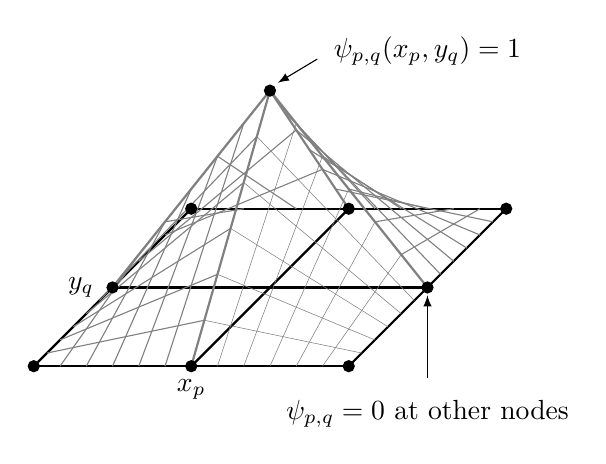
\begin{tikzpicture}[scale=0.5]

  % strong grid around elements
  \draw[thick] (0,0) -- (8,0);
  \draw[thick] (2,2) -- (10,2);
  \draw[thick] (4,4) -- (12,4);
  \draw[thick] (0,0) -- (4,4);
  \draw[thick] (4,0) -- (8,4);
  \draw[thick] (8,0) -- (12,4);

  \def\ytop{7};

  % tent lines
  \draw[gray,thick] (6,\ytop) -- (4,0);
  \draw[gray,thick] (6,\ytop) -- (2,2);
  \draw[gray,thick] (6,\ytop) -- (10,2);
  \draw[gray,thick] (6,\ytop) -- (8,4);

  \def\dx{(10.0-6.0)/6};
  \def\dy{(2.0-\ytop)/6};
  \foreach \jj in {1,...,5}
  {
       \draw[gray,very thin] ({6+\jj*\dx},{\ytop+\jj*\dy}) -- ({4+(4/6)*\jj},0.0);
  }

  \def\dx{(4.0-6.0)/6};
  \def\dy{(0.0-\ytop)/6};
  \foreach \jj in {1,...,5}
  {
       \draw[gray,very thin] ({6+\jj*\dx},{\ytop+\jj*\dy}) -- ({10-(2/6)*\jj},{2-(2/6)*\jj});
  }

  \def\dx{(2.0-6.0)/6};
  \def\dy{(2.0-\ytop)/6};
  \foreach \jj in {1,...,5}
  {
       \draw[gray,thin] ({6+\jj*\dx},{\ytop+\jj*\dy}) -- ({4-(4/6)*\jj},0.0);
  }

  \def\dx{(4.0-6.0)/6};
  \def\dy{(0.0-\ytop)/6};
  \foreach \jj in {1,...,5}
  {
       \draw[gray,thin] ({6+\jj*\dx},{\ytop+\jj*\dy}) -- ({2-(2/6)*\jj},{2-(2/6)*\jj});
  }

  \def\dx{(10.0-6.0)/6};
  \def\dy{(2.0-\ytop)/6};
  \foreach \jj in {1,...,5}
  {
       \draw[gray,thin] ({6+\jj*\dx},{\ytop+\jj*\dy}) -- ({8+(4/6)*\jj},4.0);
  }

  \def\dx{(8.0-6.0)/6};
  \def\dy{(4.0-\ytop)/6};
  \foreach \jj in {1,...,5}
  {
       \draw[gray,thin] ({6+\jj*\dx},{\ytop+\jj*\dy}) -- ({10+(2/6)*\jj},{2+(2/6)*\jj});
  }

  \def\dx{(2.0-6.0)/3};
  \def\dy{(2.0-\ytop)/3};
  \foreach \jj in {1,...,2}  % reduce clutter
  {
       \draw[gray,thin] ({6+\jj*\dx},{\ytop+\jj*\dy}) -- ({8-(4/3)*\jj},4.0);
  }

  \def\dx{(8.0-6.0)/3};
  \def\dy{(4.0-\ytop)/3};
  \foreach \jj in {1,...,2}
  {
       \draw[gray,thin] ({6+\jj*\dx},{\ytop+\jj*\dy}) -- ({2+(2/3)*\jj},{2+(2/3)*\jj});
  }

  % nodes in base plane
  \filldraw (0,0) circle (4pt);
  \filldraw (4,0) circle (4pt);
  \filldraw (8,0) circle (4pt);
  \filldraw (2,2) circle (4pt);
  %\filldraw (6,2) circle (4pt);   % (x_j,y_k) is at (6,2)
  \filldraw (10,2) circle (4pt);
  \filldraw (4,4) circle (4pt);
  \filldraw (8,4) circle (4pt);
  \filldraw (12,4) circle (4pt);

  % node at tent top
  \filldraw (6,\ytop) circle (4pt);

  % annotate
  \draw (10,\ytop+1.0) node {$\psi_{p,q}(x_p,y_q)=1$};
  \draw[-latex] (7.2,\ytop+0.8) -- (6.2,\ytop+0.2);
  \draw (10,-1.2) node {$\psi_{p,q}=0$ at other nodes};
  \draw[-latex] (10,-0.3) -- (10,1.8);

  % label center point
  \draw (4,-0.6) node {$x_p$};
  \draw (1.2,2) node {$y_q$};

\end{tikzpicture}

\caption{FIXME}
\label{fig:q1hat}
\end{marginfigure}

FIXME code uses \texttt{SNESSetObjective()} only, though also \texttt{SNESSetFunction()}; no hand-made Jacobian at all

FIXME try NCG
